% 2018 江苏 18 图：椭圆 x^2/4+y^2=1 与圆 x^2+y^2=3（以 F1F2 为直径），F1(-√3,0)，F2(√3,0)，O(0,0)。
% 全局数值坐标，单位 1.5cm，线宽 .6pt，12pt。
\usetikzlibrary{arrows.meta,calc}
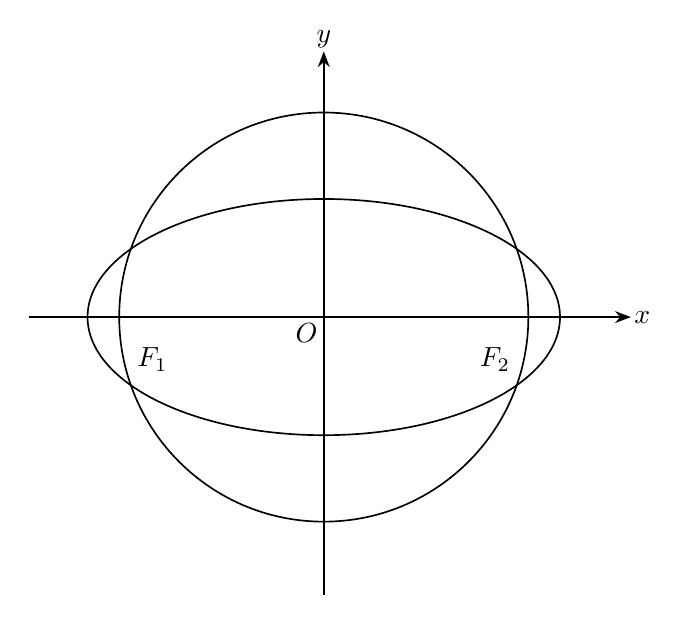
\begin{tikzpicture}[x=1.5cm,y=1.5cm,line width=.6pt,>=Stealth,font=\normalsize]
\coordinate (O) at (0,0);
\coordinate (F1) at (-1.732051,0);
\coordinate (F2) at (1.732051,0);
\draw[->] (-2.5,0)--(2.6,0) node[right,inner sep=1pt] {$x$};
\draw[->] (0,-2.35)--(0,2.25) node[above,inner sep=1pt] {$y$};
\draw (O) circle [radius=2.598076cm];
\draw (O) ellipse [x radius=3cm, y radius=1.5cm];
\node[inner sep=1pt] at (-1.45,-0.36) {$F_1$};
\node[inner sep=1pt] at (1.45,-0.36) {$F_2$};
\node[anchor=north east,inner sep=0pt,xshift=-2pt,yshift=-2pt] at (O) {$O$};
\end{tikzpicture}
